\documentclass[10pt]{beamer}\usepackage[]{graphicx}\usepackage[]{color}
%% maxwidth is the original width if it is less than linewidth
%% otherwise use linewidth (to make sure the graphics do not exceed the margin)
\makeatletter
\def\maxwidth{ %
  \ifdim\Gin@nat@width>\linewidth
    \linewidth
  \else
    \Gin@nat@width
  \fi
}
\makeatother

\definecolor{fgcolor}{rgb}{0.345, 0.345, 0.345}
\newcommand{\hlnum}[1]{\textcolor[rgb]{0.686,0.059,0.569}{#1}}%
\newcommand{\hlstr}[1]{\textcolor[rgb]{0.192,0.494,0.8}{#1}}%
\newcommand{\hlcom}[1]{\textcolor[rgb]{0.678,0.584,0.686}{\textit{#1}}}%
\newcommand{\hlopt}[1]{\textcolor[rgb]{0,0,0}{#1}}%
\newcommand{\hlstd}[1]{\textcolor[rgb]{0.345,0.345,0.345}{#1}}%
\newcommand{\hlkwa}[1]{\textcolor[rgb]{0.161,0.373,0.58}{\textbf{#1}}}%
\newcommand{\hlkwb}[1]{\textcolor[rgb]{0.69,0.353,0.396}{#1}}%
\newcommand{\hlkwc}[1]{\textcolor[rgb]{0.333,0.667,0.333}{#1}}%
\newcommand{\hlkwd}[1]{\textcolor[rgb]{0.737,0.353,0.396}{\textbf{#1}}}%
\let\hlipl\hlkwb

\usepackage{framed}
\makeatletter
\newenvironment{kframe}{%
 \def\at@end@of@kframe{}%
 \ifinner\ifhmode%
  \def\at@end@of@kframe{\end{minipage}}%
  \begin{minipage}{\columnwidth}%
 \fi\fi%
 \def\FrameCommand##1{\hskip\@totalleftmargin \hskip-\fboxsep
 \colorbox{shadecolor}{##1}\hskip-\fboxsep
     % There is no \\@totalrightmargin, so:
     \hskip-\linewidth \hskip-\@totalleftmargin \hskip\columnwidth}%
 \MakeFramed {\advance\hsize-\width
   \@totalleftmargin\z@ \linewidth\hsize
   \@setminipage}}%
 {\par\unskip\endMakeFramed%
 \at@end@of@kframe}
\makeatother

\definecolor{shadecolor}{rgb}{.97, .97, .97}
\definecolor{messagecolor}{rgb}{0, 0, 0}
\definecolor{warningcolor}{rgb}{1, 0, 1}
\definecolor{errorcolor}{rgb}{1, 0, 0}
\newenvironment{knitrout}{}{} % an empty environment to be redefined in TeX

\usepackage{alltt}
% \usetheme{jhsph}
\usepackage[T1]{fontenc}
\setcounter{secnumdepth}{3}
\setcounter{tocdepth}{3}
\usepackage{url}
\usepackage{graphicx}
\usepackage{multimedia}
\ifx\hypersetup\undefined
  \AtBeginDocument{%
    \hypersetup{unicode=true,pdfusetitle,
 bookmarks=true,bookmarksnumbered=false,bookmarksopen=false,
 breaklinks=false,pdfborder={0 0 0},pdfborderstyle={},backref=false,colorlinks=false}
  }
\else
  \hypersetup{unicode=true,pdfusetitle,
 bookmarks=true,bookmarksnumbered=false,bookmarksopen=false,
 breaklinks=false,pdfborder={0 0 0},pdfborderstyle={},backref=false,colorlinks=false}
\fi
\usepackage{breakurl}

\makeatletter

%%%%%%%%%%%%%%%%%%%%%%%%%%%%%% Textclass specific LaTeX commands.
 % this default might be overridden by plain title style
 \newcommand\makebeamertitle{\frame{\maketitle}}%
 % (ERT) argument for the TOC
 \AtBeginDocument{%
   \let\origtableofcontents=\tableofcontents
   \def\tableofcontents{\@ifnextchar[{\origtableofcontents}{\gobbletableofcontents}}
   \def\gobbletableofcontents#1{\origtableofcontents}
 }


\newcommand\blfootnote[1]{%
  \begingroup
  \renewcommand\thefootnote{}\footnote{#1}%
  \addtocounter{footnote}{-1}%
  \endgroup
}

\usetheme{PaloAlto}

\makeatother
\IfFileExists{upquote.sty}{\usepackage{upquote}}{}
\begin{document}

\title[]{Joint modeling of daily patterns of heart rate and physical activity data: Estimating individual heterogeneity in physiologic response to physical activity}
% \subtitle[]{Analyzing ``macro" scale accelerometry data: NHANES}
\author[]{Andrew Leroux}
\makebeamertitle


% \section{Background}


% \section{Wearable and Implantable Technology}


\section{Background}




\begin{frame}
\frametitle{Motivation}
\begin{itemize}
\item the ``\textbf{big}" questions: 
    \begin{enumerate}
    \item What is the effect of physical activity (PA) on heart rate (HR)? 
    \item Can we quantify individual heterogeneity in this effect adjusting for age, health status, and diurnal patterns of both PA and HR? 
    \item Is this individual heterogeneity associated with outcomes of interest? 
    \end{enumerate}
\item Challenges:
    \begin{itemize}
    \item Need (good) data (lots of it)
    \item Normalize for differences in capacity (``maximum" and resting heart rate)
    \item What is a sensible statistical model?
    \end{itemize}
\end{itemize}
\end{frame}

\begin{frame}
\frametitle{Data}
\begin{itemize}
\item Baltimore Longitudinal Study on Aging (BLSA) 
\item Actiheart - chest worn uniaxial accelerometer and heart rate monitor 
\item Exclusion criteria
        \begin{itemize}
        \item Ages 30-90
        \item Peak respiratory exchange ratio $\geq 1.1$ 
        \item Estimated VO$_2$ max $\geq 10$ 
        \item No missing data for demographic variables, several comorbidities, and alcohol consumption
        \item At least 3 days of ``good" Actiheart data
        \item No beta blockers
        \end{itemize}
\item Final sample: $446$ subjects, 233 male and 213 female 
\end{itemize}
\end{frame}



\section{PA, HR, and HRR}

\begin{frame}
\frametitle{Defining Activity Intensity Using Heart Rate Reserve}

\begin{equation*}
\text{Heart Rate Reserve} = \text{Maximum Heart Rate} - \text{Resting Heart Rate}
\end{equation*}

\begin{center}
\begin{tabular}{ll}
Vigorous:& 60\% or greater of HRR over resting  \\
Moderate:& 40-59\%  \\ 
Light:&    20-39\% \\
Sedentary:& <20\%
\end{tabular}
\end{center}

We can approximate maximum heart rate using observed maximum heart rate from the treadmill test, but
we need to estimate resting heart rate.

\end{frame}


\begin{frame}\frametitle{Estimating Resting Heart Rate}

Resting heart rate estimation algorithm: 

\begin{center}
\small
\begin{tabular}{ll} \hline \hline
Step 1:& Examine 5 minute moving windows to find all 10-minute intervals \\
       & between 01:00-07:00 with 0 total activity counts  \\ \hline
Step 2:& Calculate average heart rate of the last 5 minutes of each interval   \\ 
       & found in (1) \\ \hline
Step 3:& Take the average of the heart rates found in (2) \\ \hline \hline
\end{tabular}
\end{center}


\end{frame}



\begin{frame}\frametitle{Estimating Resting Heart Rate}
\begin{center}
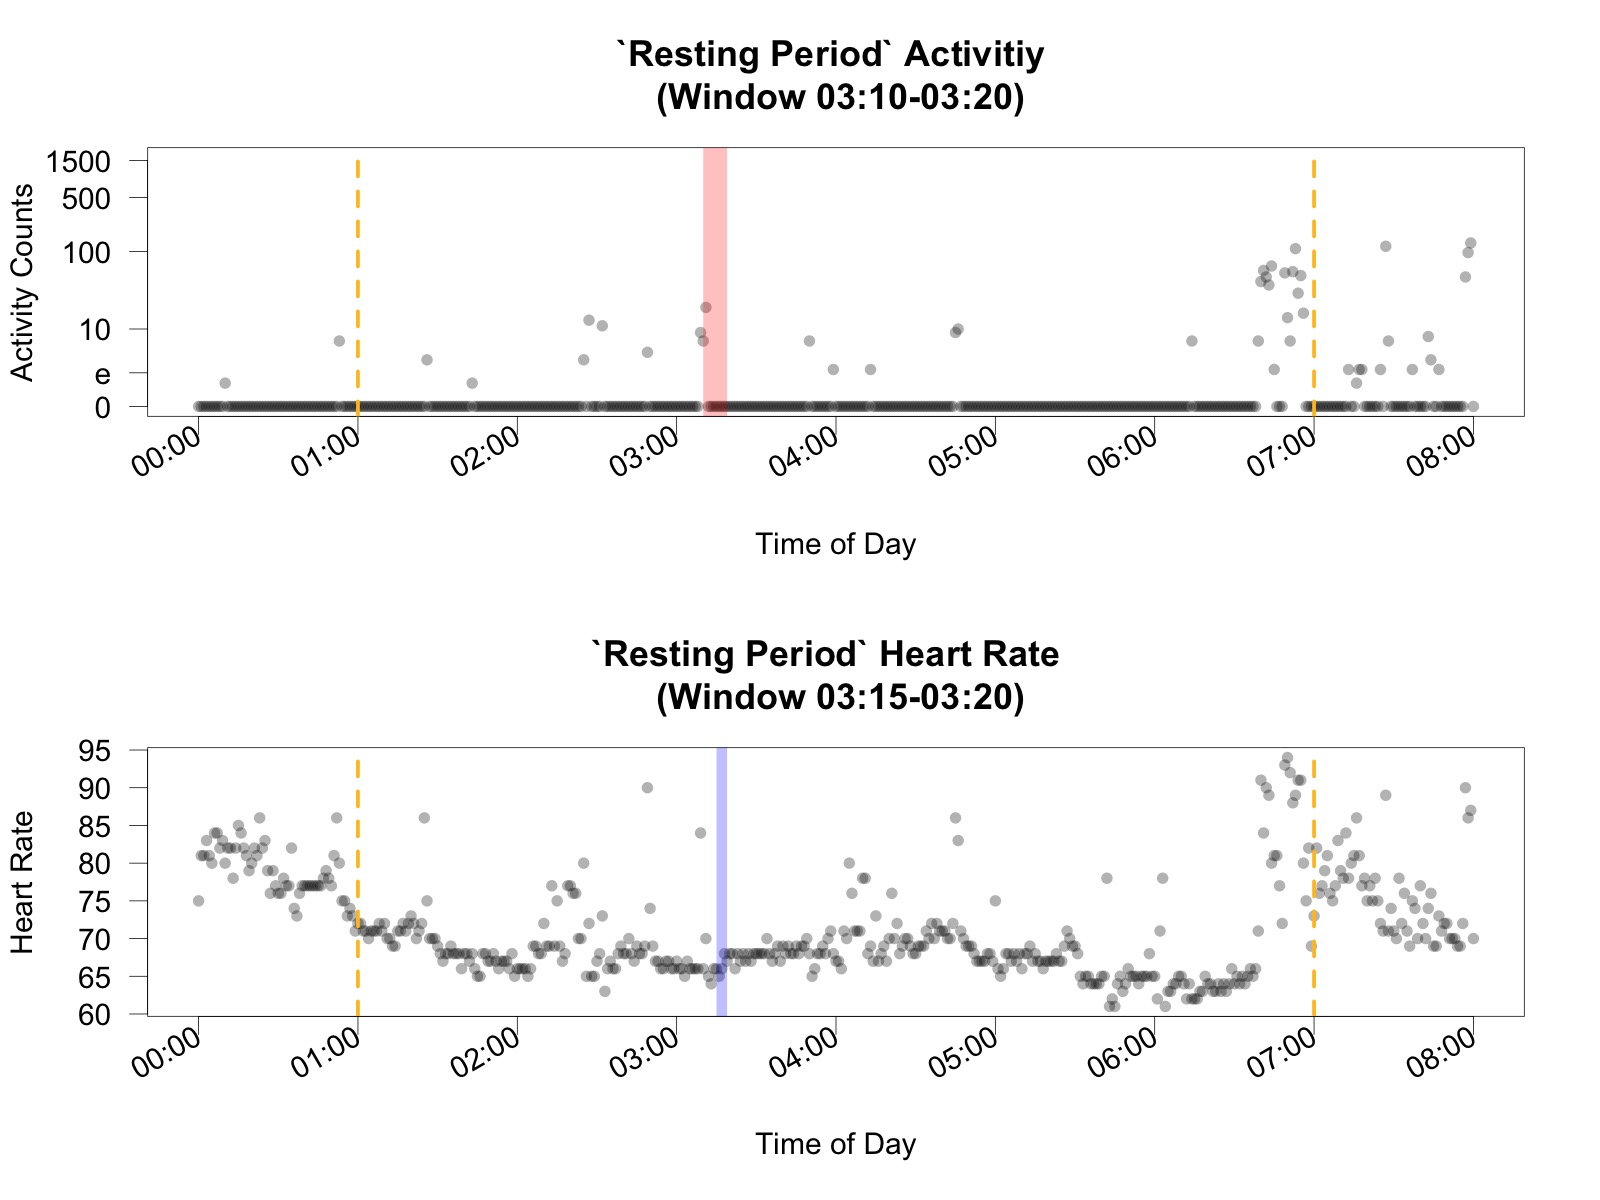
\includegraphics[scale=0.15]{RestingHeartRate_P3.jpeg}
\end{center}
\end{frame}


\begin{frame}\frametitle{Estimating Resting Heart Rate}
\begin{center}
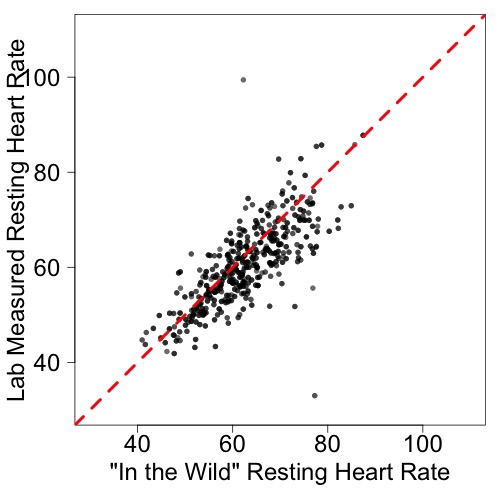
\includegraphics[height=\textheight]{resting_est_wild.jpeg}
\end{center}
\end{frame}

\begin{frame}\frametitle{Estimating Resting Heart Rate}
\begin{center}
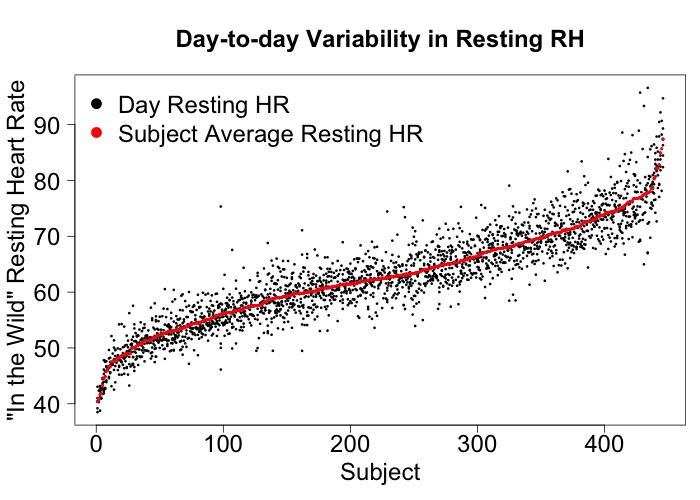
\includegraphics[width=\textwidth]{resting_est_wild_day_to_day.jpeg}
\end{center}
\end{frame}




\begin{frame}\frametitle{Estimated Heart Rate Reserve: $HRR(t)$}
57M, healthy, 37 peak VO$_2$, 163 max HR
\begin{center}
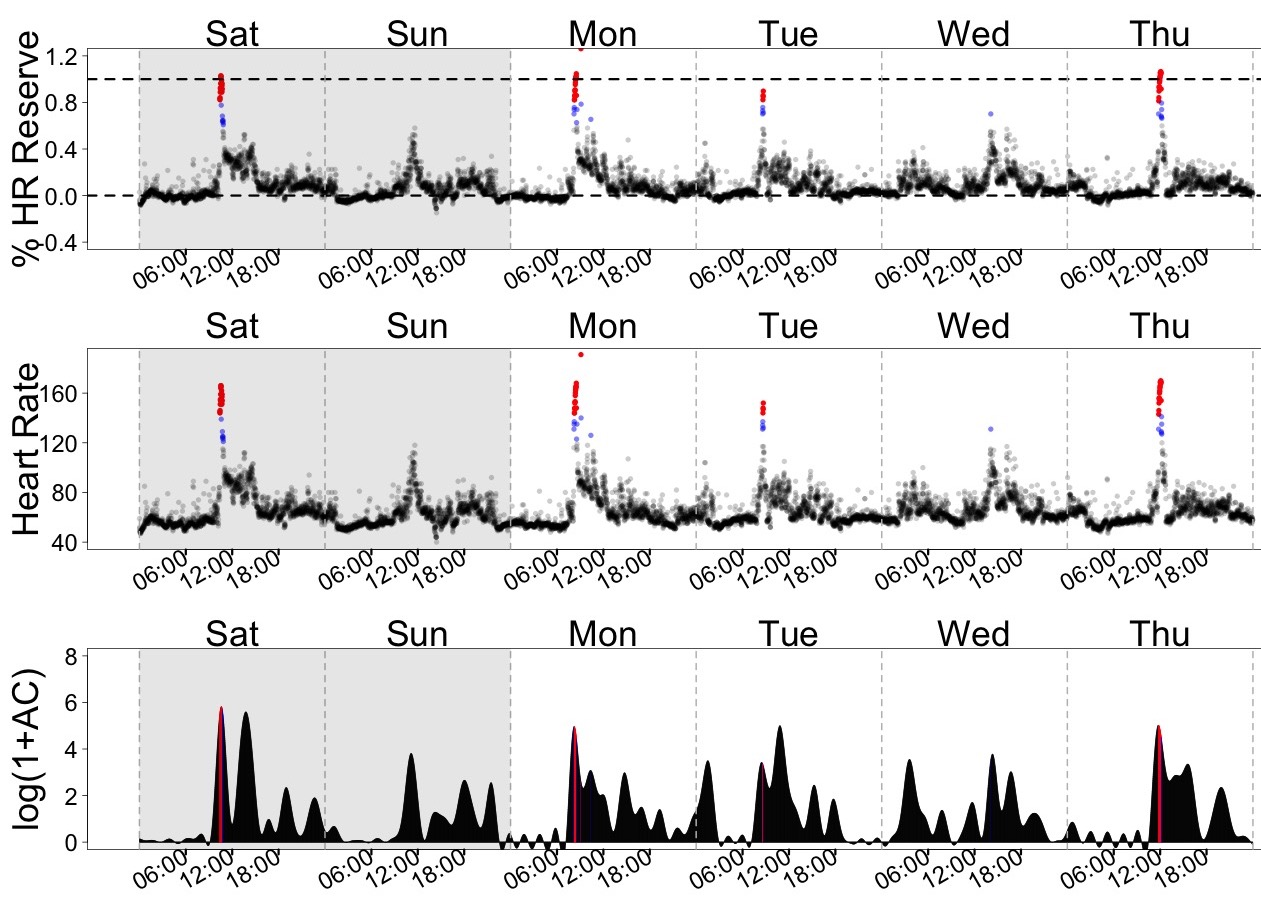
\includegraphics[width=\textwidth]{AC_HRR_HR_subj_4952}
\end{center}
\end{frame}

\begin{frame}\frametitle{Estimated Heart Rate Reserve: $HRR(t)$}
70F, healthy, 20 VO$_2$, 163 max HR
\begin{center}
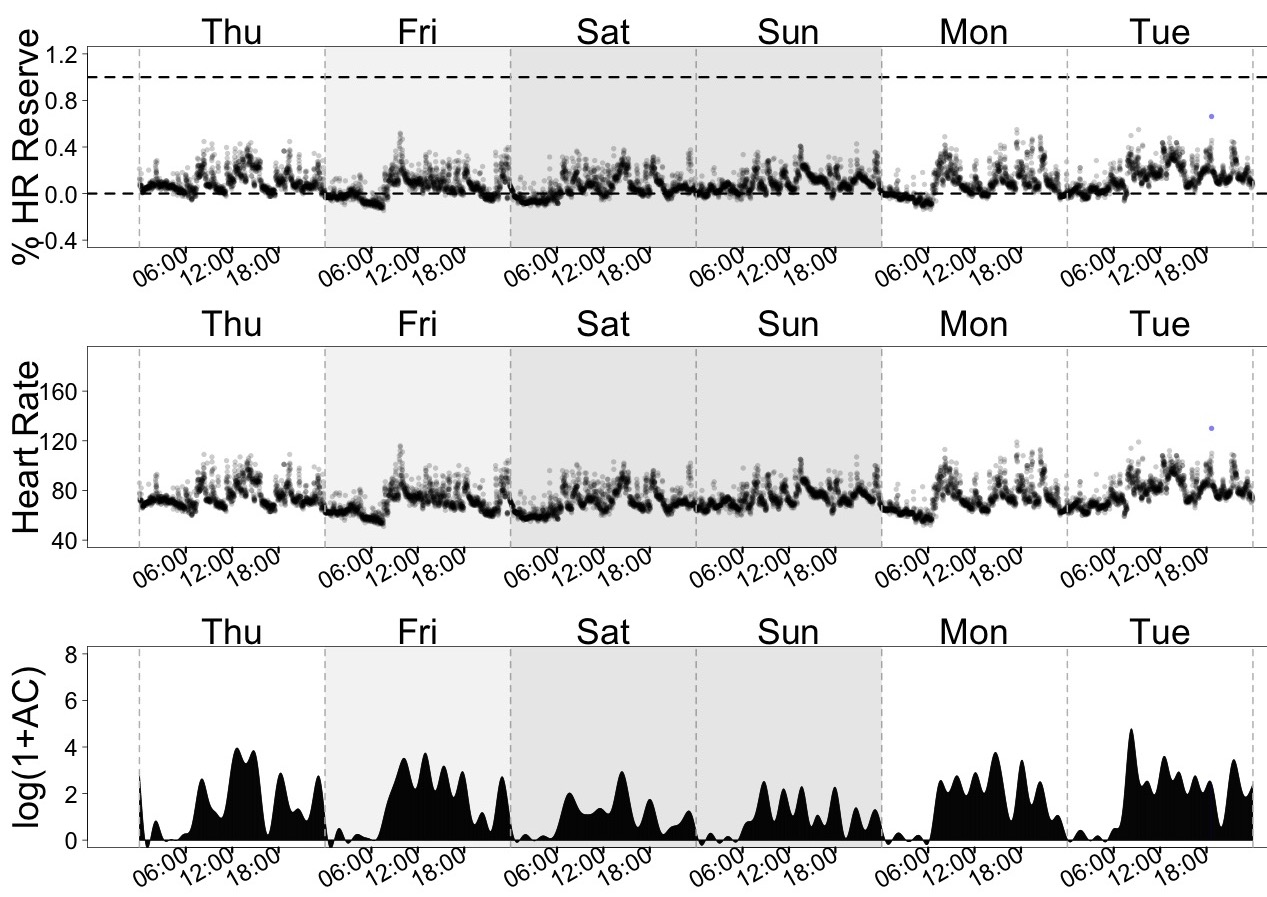
\includegraphics[width=\textwidth]{AC_HRR_HR_subj_7774}
\end{center}
\end{frame}


\begin{frame}\frametitle{Estimated Heart Rate Reserve: $HRR(t)$}
82M, cancer, 18 peak VO$_2$, 127 max HR, 9 borg scale
\begin{center}
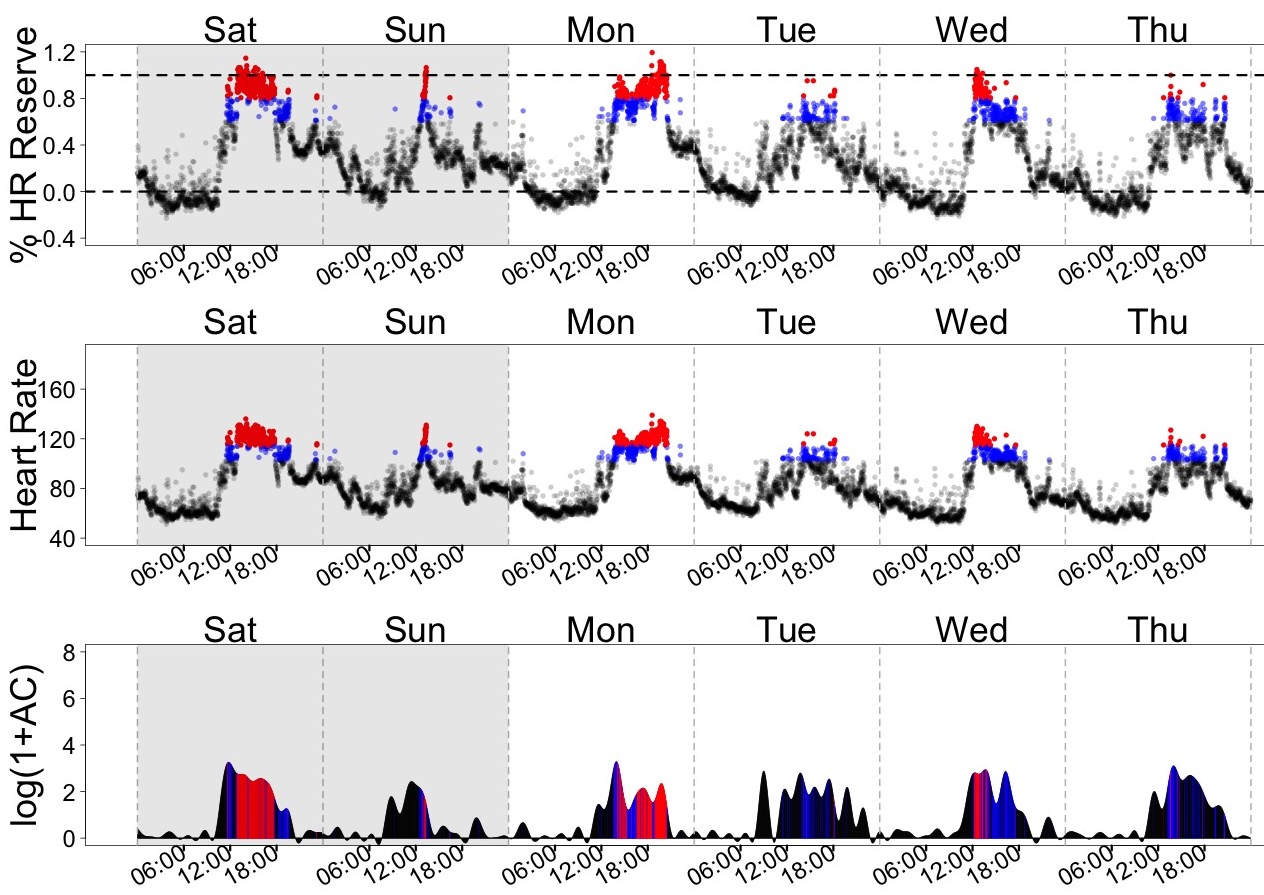
\includegraphics[width=\textwidth]{AC_HRR_HR_subj_4832}
\end{center}
\end{frame}

\begin{frame}\frametitle{Estimated Heart Rate Reserve: $HRR(t)$}
74F, hypertension,  cancer, 16 VO$_2$, 89 max HR, 13 borg scale
\begin{center}
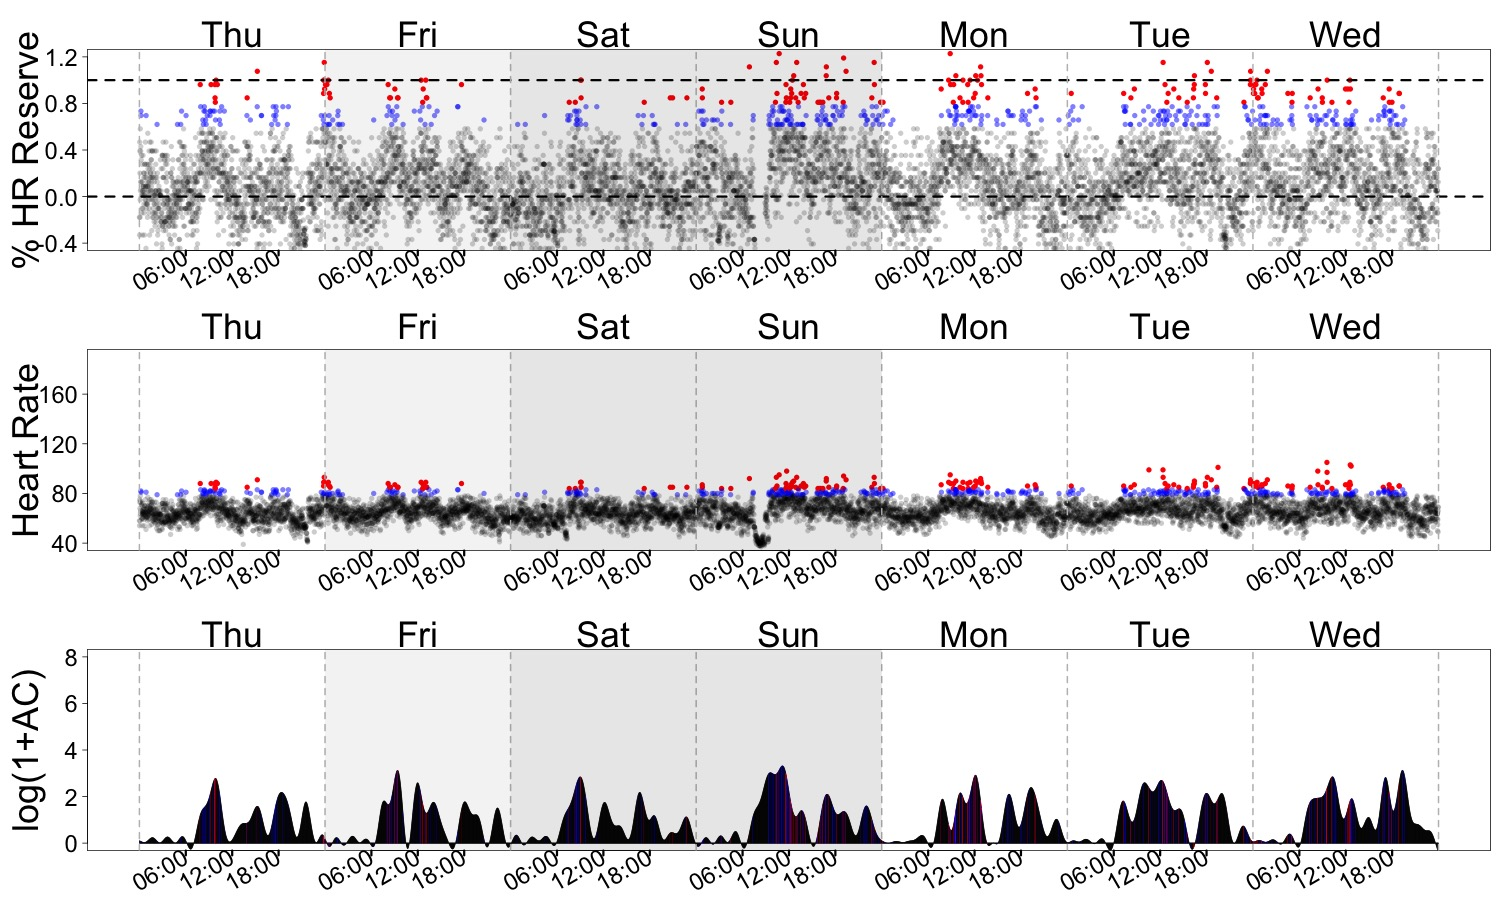
\includegraphics[width=\textwidth]{AC_HRR_HR_subj_5614}
\end{center}
\end{frame}




\subsection{Marginal Models}



\begin{frame}
\frametitle{PA, HR, and HRR vs Age}
\begin{itemize}
\item Model daily patterns of PA, HR, and HRR as a function of age
\item Fit 3 separate models:
\begin{align*}
E[Y_{ij}(t)|\mathbf{X}_i, \text{Age}_i, t] &= f_0(t) + \sum_{p=1}^P X_{ip}f_p(t) + \beta(\text{Age}_i,t)
\end{align*}
\item $i = 1,\ldots,N$ subject, $j= 1,\ldots,J_i$ day, $t = 1,\ldots,1440$ minute of the day
\item $X_{ip}$ are scalar covariates (BMI, comorbidities, etc.)
\item $\beta(\text{Age}_i,t)$ allows for outcome to vary smoothly in time and age
\end{itemize}
\end{frame}



\begin{frame}
\frametitle{PA vs Age}
\begin{center}
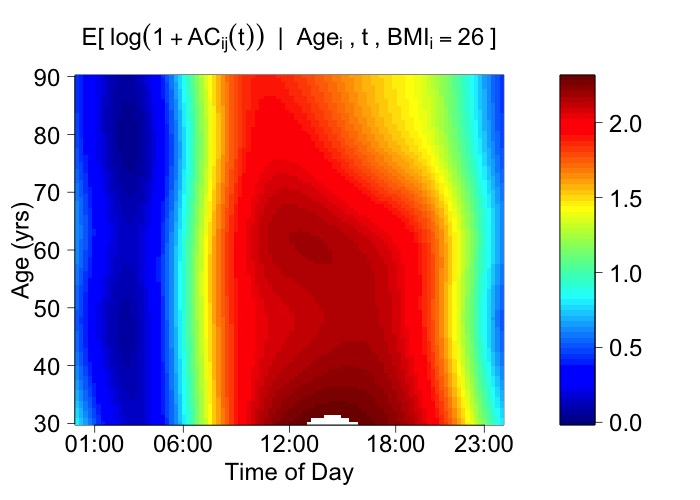
\includegraphics[height=\textheight]{coef_AC_mar.jpeg}
\end{center}
\end{frame}

\begin{frame}
\frametitle{HR vs Age}
\begin{center}
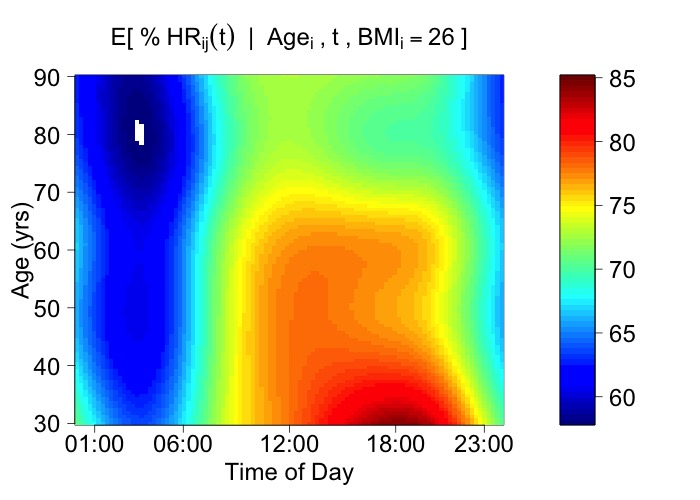
\includegraphics[height=\textheight]{coef_HR_mar.jpeg}
\end{center}
\end{frame}

\begin{frame}
\frametitle{HRR vs Age}
\begin{center}
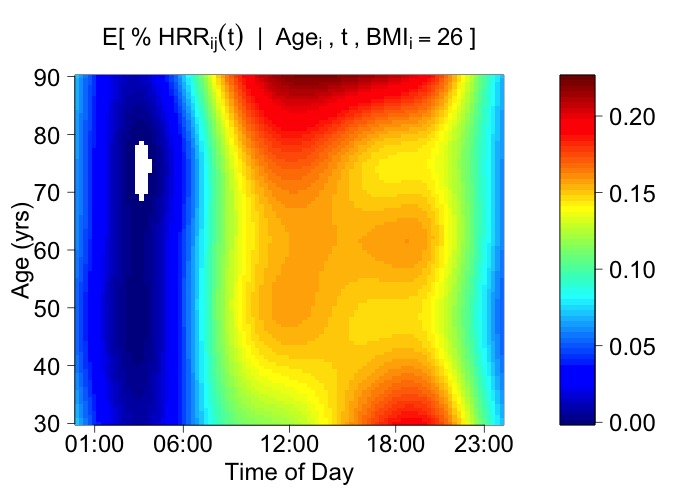
\includegraphics[height=\textheight]{coef_HRR_mar.jpeg}
\end{center}
\end{frame}


\begin{frame}
\frametitle{PA, HR, and HRR vs Age}
\begin{center}
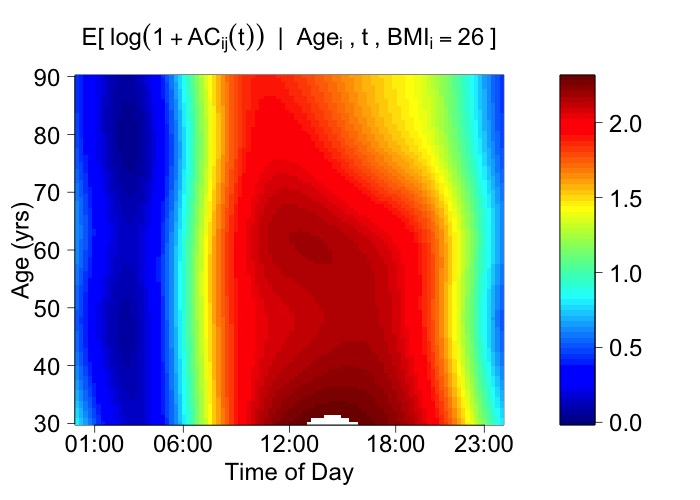
\includegraphics[width=0.5\textwidth]{coef_AC_mar.jpeg}
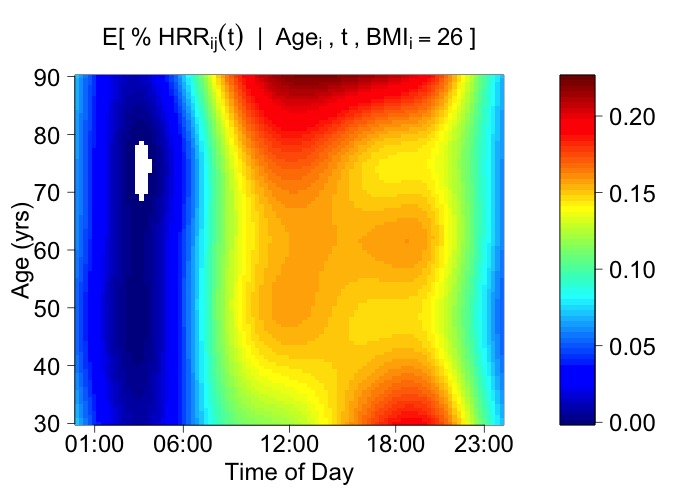
\includegraphics[width=0.5\textwidth]{coef_HRR_mar.jpeg}
\end{center}
\end{frame}



\begin{frame}
\frametitle{PA, HR, and HRR vs Age}
\begin{itemize}
\item Attempt to adjust for PA at a given time
\begin{align*}
E[\text{HRR}_{ij}(t)|\cdot] &= f_0(t) + \sum_{p=1}^P X_{ip}f_p(t) + \beta(\text{Age}_i,t) + \gamma_1(t)\text{LAC}_{ij}(t)
\end{align*}
\item Concurrent effect of activity on heart rate
\item Historical effect of PA?
\end{itemize}
\end{frame}



\begin{frame}
\frametitle{HRR adjusting for PA}
\begin{center}
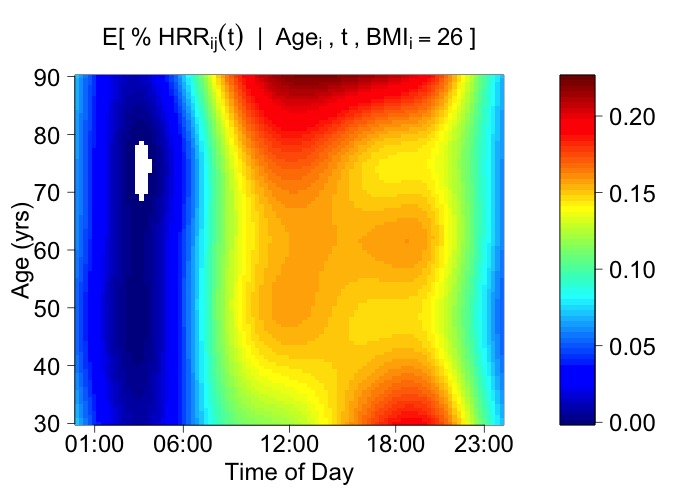
\includegraphics[width=0.5\textwidth]{coef_HRR_mar.jpeg}
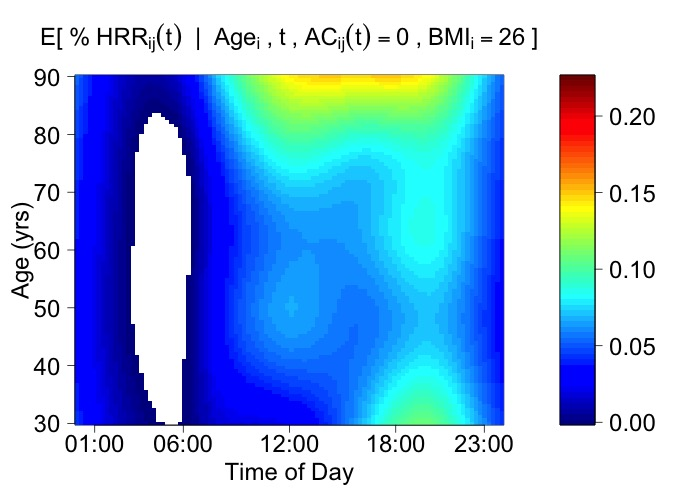
\includegraphics[width=0.5\textwidth]{coef_HRR_lAC0.jpeg}
\end{center}
\end{frame}






\subsection{Subject Specific Effects}

\begin{frame}
\frametitle{PA, HR, and HRR vs Age}
\begin{itemize}
\item HRR at rest will vary from person-to-person (latent health status) and day-to-day (hydration, mental state, etc.) 
\item For now ignore day-to-day variability \pause
\begin{align*}
\text{HRR}_{ij}(t) &= \eta_{i}(t) + \gamma(t)\text{LAC}_{ij}(t) + b_{0i}(t) +  b_{1ij}(t)\text{LAC}_{ij}(t) + \epsilon_{ij}(t)
\end{align*}
\item $\eta_{i}(t) = f_0(t) + \sum_{p=1}^P X_{ip}f_p(t) + \beta(\text{Age}_i,t) $
\item $b_{0i}(t)$ represents subject $i$'s average HRR difference from the population at rest
\item {\color{red}$b_{1i}(t)$} represents subject $i$'s deviation from the population in response to PA
\end{itemize}
\end{frame}


\begin{frame}
\frametitle{Estimating $b_{1i}(t)$}
\begin{itemize}
\item How to estimate subject specific responses? 
    \begin{enumerate}
        \item Fit marginal model, obtain residuals, fit $N$ separate regressions
        \item Fit marginal model, obtain residuals, GLS, fit $N$ separate regressions
        \item Fit the ``full" model (functional mixed effects model)
    \end{enumerate}
\item Choice of estimation procedure depends on goals.
\end{itemize}
\end{frame}


\begin{frame}
\frametitle{Estimating $b_{1i}(t)$}
\begin{center}
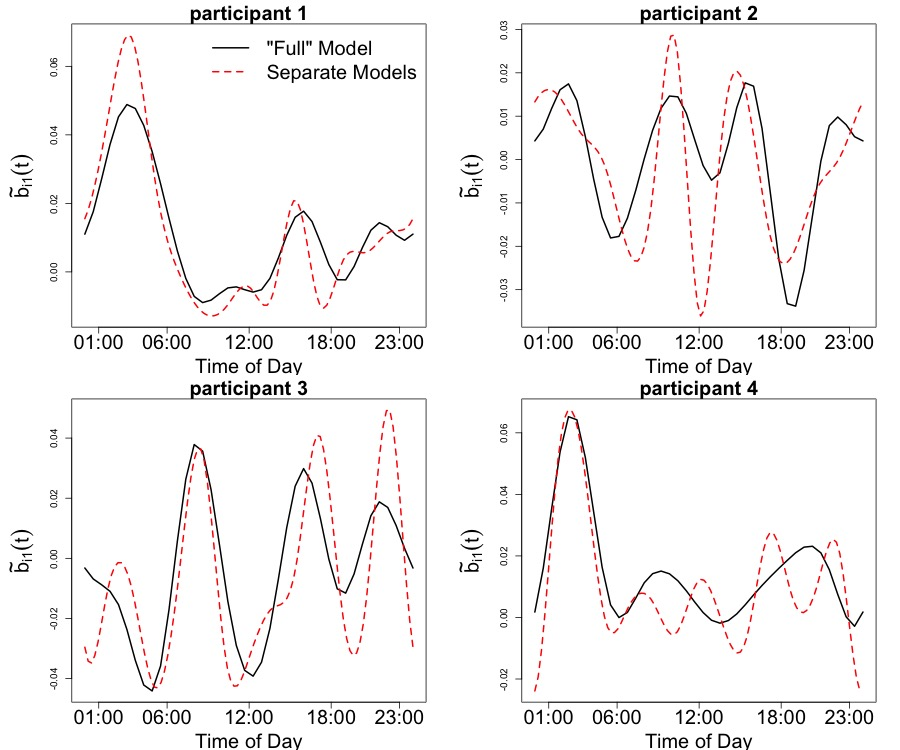
\includegraphics[width=\textheight]{re_subjs2.jpeg}
\end{center}
\end{frame}

\begin{frame}
\frametitle{Using Estimated $\tilde{b}_{1i}(t)$}
\begin{itemize}
\item $\tilde{b}_{1i}(t)$ as a functional predictor 
\item scalar summary (e.g. $\int_T \tilde{b}_{1i}(t)dt$, the average across the day)
\end{itemize}
\end{frame}



\section{Application: Fatigability}

\begin{frame}
\frametitle{Fatigability}
\begin{center}
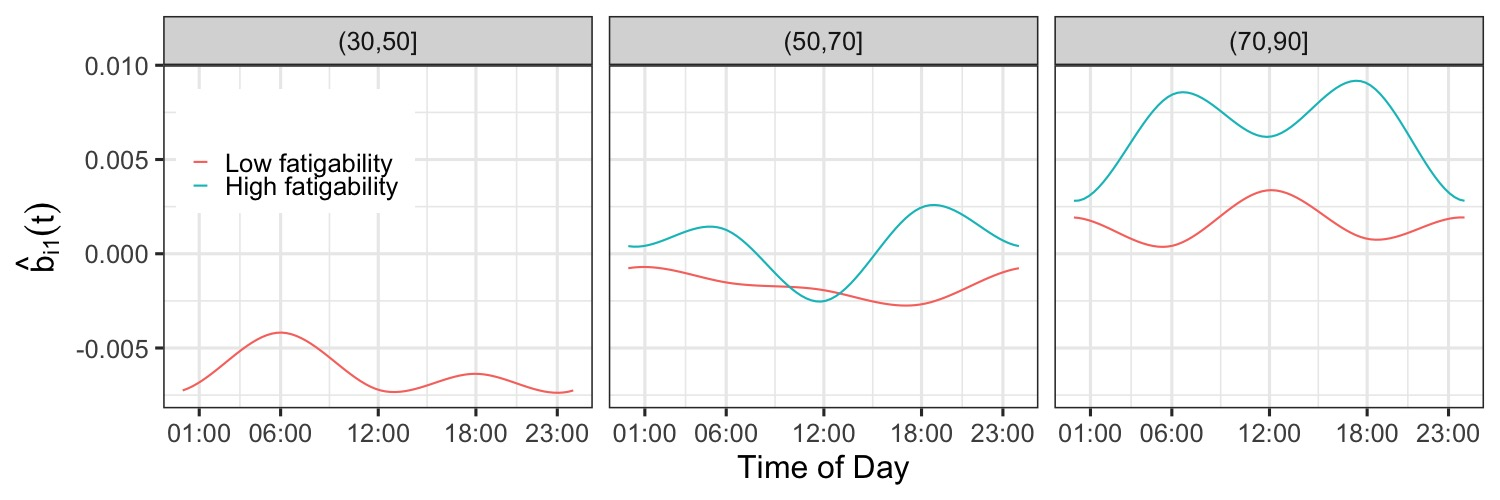
\includegraphics[width=\textwidth]{bi2_by_age_tss.jpeg}
\end{center}
\end{frame}

\begin{frame}
\frametitle{Fatigability}
\begin{center}
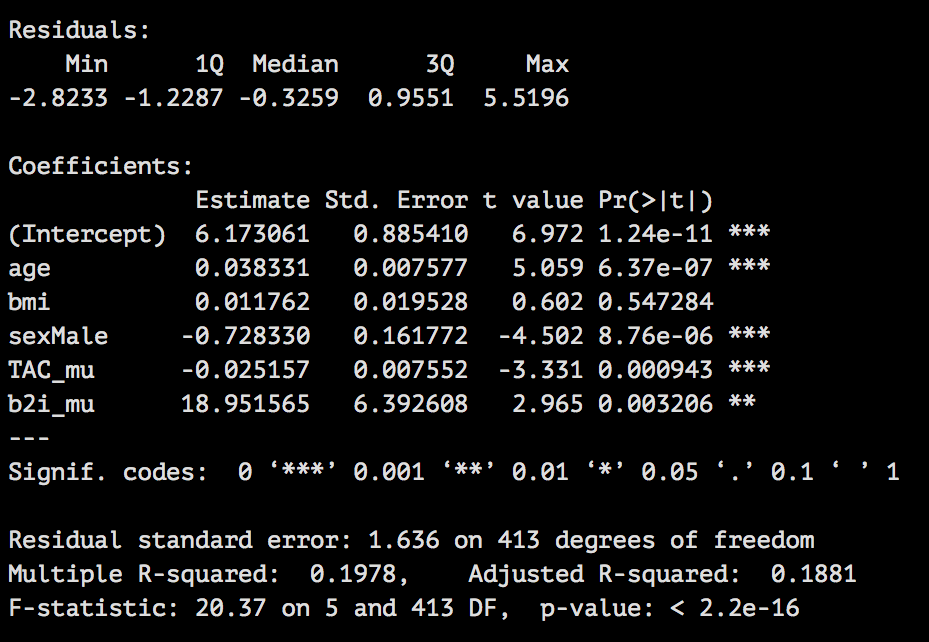
\includegraphics[width=\textwidth]{lm_borg}
\end{center}
\end{frame}


\section{Future Work}


\begin{frame}
\frametitle{Next steps/Open questions}
\begin{itemize}
\item What does it mean when $\gamma(t) + b_{i1}(t) \leq 0$? Individual thresholds? Bad data?
\item Day-to-day variability? 
\item Building in a historical effect of activity (of heart rate?)
\end{itemize}
\end{frame}


\section{Scalar on Function Regression}



\begin{frame}
\frametitle{Scalar on Function Regression}

\begin{itemize}
\item Scalar on function regression can take many forms

\item \textbf{Functional Generalized Linear Model\footnotemark (FGLM):} Association varies with time of day, but scales linearly with (log) activity count
\begin{align*}
g(E[Y_i]) &= X_i^\prime\beta + \int_T f(t)Z_i(t)dt 
\end{align*}

\item \textbf{Functional Generalized Additive Model\footnotemark (FGAM):}  Association varies smoothly with both time of day and value of (log) activity count
\begin{align*}
g(E[Y_i]) &= X_i^\prime\beta + \int_T f[t,Z_i(t)]dt
\end{align*}

\end{itemize}

\footnotetext{M\"{u}ller HG, Stadtm\"{u}ller U. Generalized functional linear models. Annals of Statistics. 2005;33(2):774-805.}
\footnotetext{McLean MW, Hooker G, Staicu AM, Scheipl F, Ruppert D. Functional Generalized Additive Models. J Comput Graph Stat. 2014;23(1):249-269.}

\end{frame}





\begin{frame}
\frametitle{Scalar on Function Regression}
\begin{itemize}

\item In both FGLR and FGAM estimation is done by applying a spline basis to the coefficient and then approximating the functional term numerically.
\begin{align*}
\int_T f(t)Z_i(t) dt &= \int_t \sum_{k=1}^K \xi_k \phi_k(t) Z_i(t) dt \hspace{0.25cm}\text{Apply spline basis} \\
&\approx \sum_l \delta_l \sum_{k=1}^K\xi_k \phi_k(l) Z_i(l) \hspace{0.25cm}\text{Numeric Approximation} \\
&= \sum_{k=1}^K\xi_k \left[\sum_l \delta_l  \phi_k(l) Z_i(l)\right]  \\
&= \sum_{k=1}^K\xi_k \tilde{Z}_i(k)  \\
\end{align*}
\item 
\end{itemize}
\end{frame}



\section{Application: Predicting Alcohol Consumption}

\begin{frame}
\frametitle{SoFR: Heavy Drinkers}
\begin{itemize}
\item Let $Y_i$ be the binary indicator that subject $i$ self reports heavy drinking
\item Logistic regression
    \begin{itemize}
    \item FGLR: $\text{logit}(p_i|X_i,\mathbf{Z}_i) = X_i^\prime \beta + \int_T f(t)Z_i(t)dt $
    \item FGAM: $\text{logit}(p_i|X_i,\mathbf{Z}_i) = X_i^\prime\beta + \int_T f[t,Z_i(t)]dt$
    \end{itemize}
\item Estimation via using {\it refund::pfr()} function
\item Adjust for linear effects of age, body mass index, and sex
\end{itemize}
\end{frame}




\begin{frame}
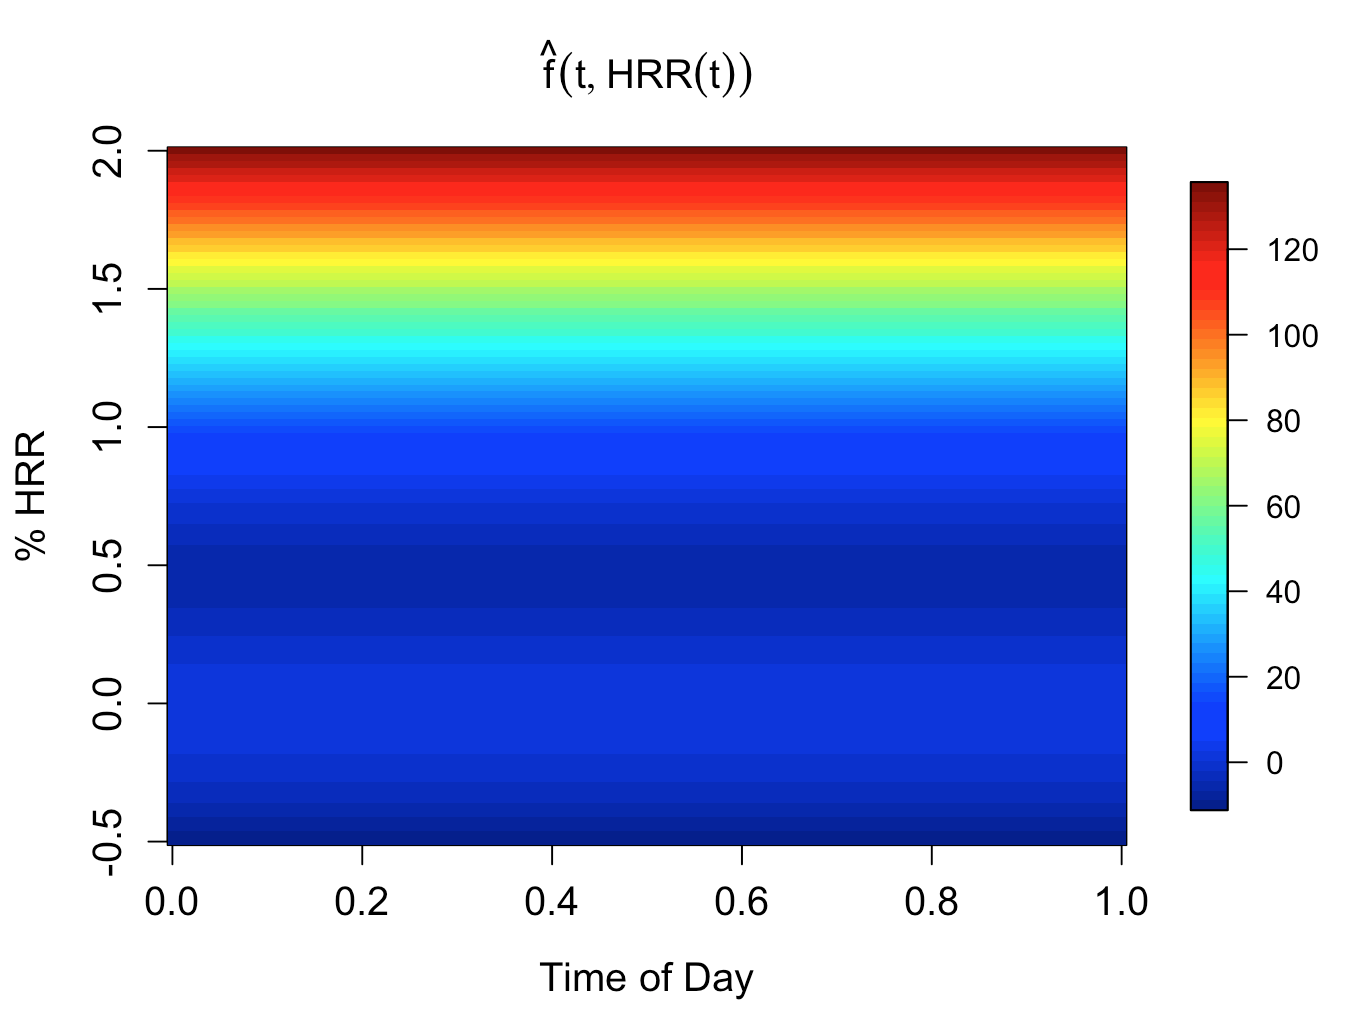
\includegraphics[height=\textheight]{fgam_hrr}
\end{frame}

\begin{frame}
\frametitle{FGAM}
\begin{itemize}
\item Estimated coefficient surface seems to imply high heart rate at any time of the is associated with increased log odds of drinking heavily
\item Very few ``high" HRR during the early morning hours
\item Consider a transformation to reduce data sparsity. Here we use the empirical CDF $\hat{g}_t(x) = \frac{1}{N}\sum_{i=1}^N I(Z_i(t) < x)$ for all $t$.
    \begin{align*}
    \text{logit}(p_i|X_i,\mathbf{Z}_i) = X_i^\prime\beta + \int_T f[t,g_t(Z_i(t))]dt
    \end{align*}
\end{itemize}
\end{frame}


\begin{frame}
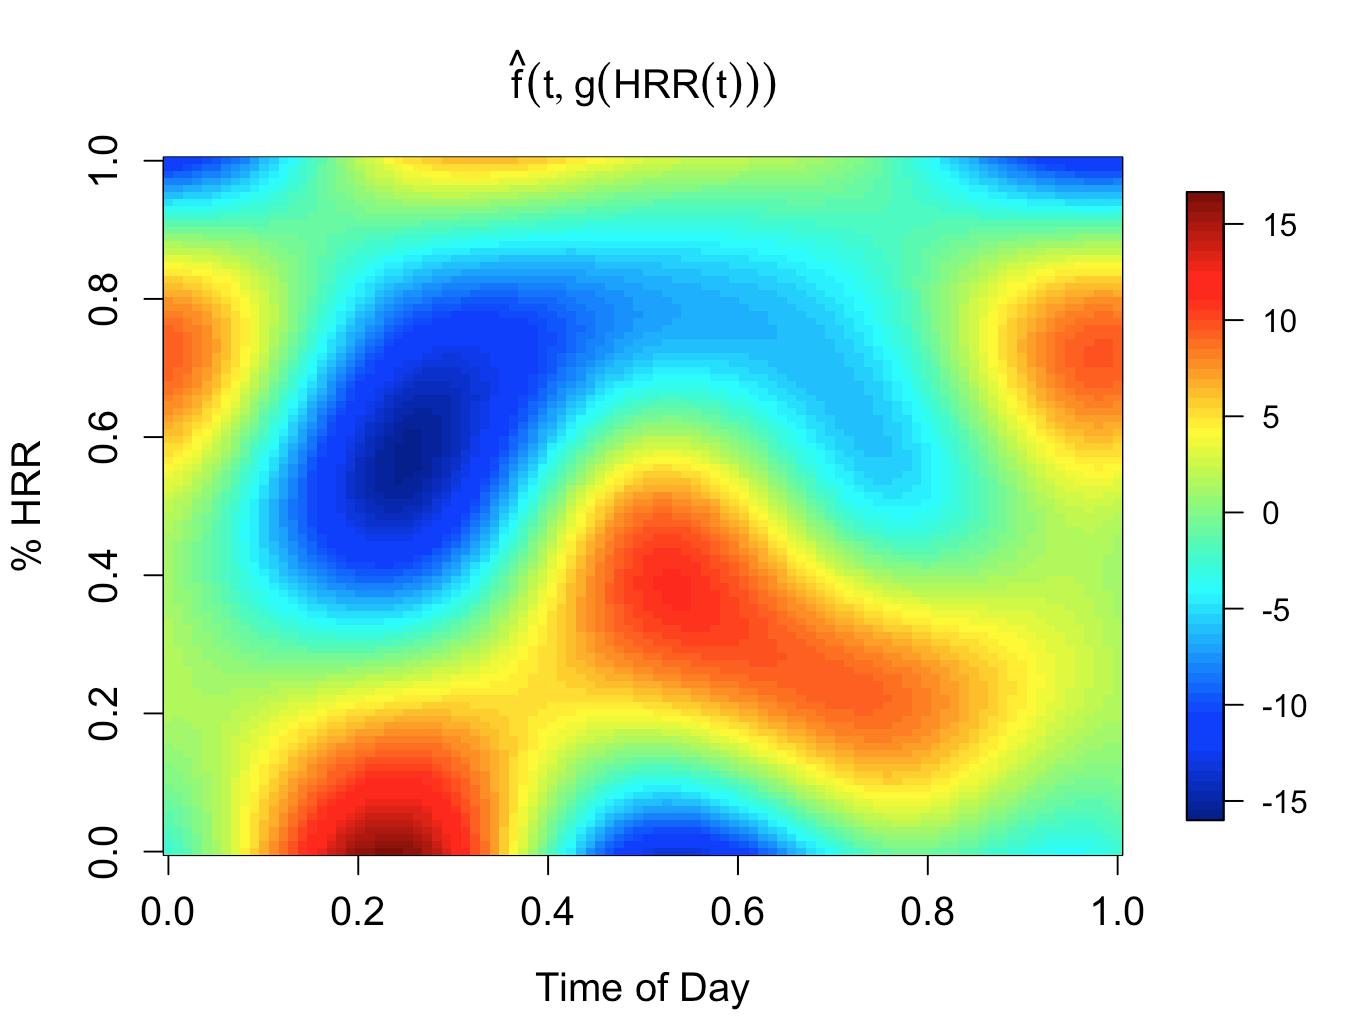
\includegraphics[height=\textheight]{fgam_hrr_q}
\end{frame}












\end{document}
